\section{Пространственная когерентность}

\begin{itemize}
	\item $|\vec{k}| = \frac{\omega}{v} = \frac{\omega}{c}n$, \quad $\frac{\vec{k}}{k} = \vec{e}_k \longrightarrow$ связана с разбросом направлений $\vec{k}$.
	
	Временная когерентность связана с разбросом $|\vec{k}|$.
\end{itemize}

\begin{figure}[H]
	\centering
	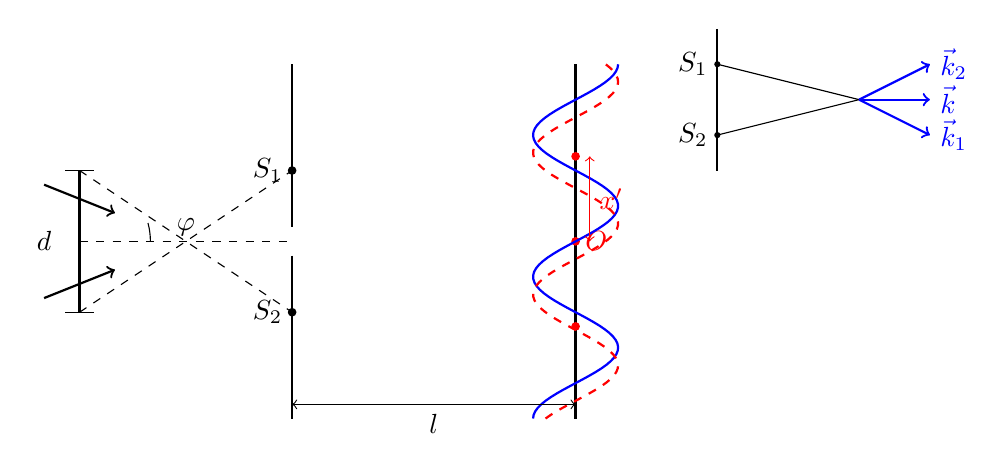
\begin{tikzpicture}[scale=0.9]
		% Source
		\draw[thick] (-3, 1) -- (-3, -1);
		\draw (-3.5, 0) node {$d$};
		\draw (-3.2, 1) -- (-2.8, 1);
		\draw (-3.2, -1) -- (-2.8, -1);
		
		% Source rays
		\draw[dashed] (-3, 0) -- (0, 0);
		\draw (-2, 0) arc (0:15:1);
		\node at (-1.5, 0.2) {$\varphi$};
		\draw[dashed] (-3, 1) -- (0, -1);
		\draw[dashed] (-3, -1) -- (0, 1);
		\draw[thick, ->] (-3.5, 0.8) -- (-2.5, 0.4);
		\draw[thick, ->] (-3.5, -0.8) -- (-2.5, -0.4);
		
		% Slits plane
		\draw[thick] (0, 2.5) -- (0, 0.2);
		\draw[thick] (0, -0.2) -- (0, -2.5);
		\filldraw (0, 1) circle (1.5pt);
		\filldraw (0, -1) circle (1.5pt);
		\node[left] at (0, 1) {$S_1$};
		\node[left] at (0, -1) {$S_2$};
		
		% Screen
		\draw[thick] (4, 2.5) -- (4, -2.5);
		\node[right, text=red] at (4, 0) {$O$};
		\filldraw[red] (4, 0) circle (1.5pt);
		\filldraw[red] (4, 1.2) circle (1.5pt);
		\filldraw[red] (4, -1.2) circle (1.5pt);
		
		% Waves on screen
		\draw[thick, blue, domain=-2.5:2.5, samples=100] plot ({4 + 0.6*cos(\x*180 - 90)}, {\x});
		\draw[thick, red, dashed, domain=-2.5:2.5, samples=100] plot ({4 + 0.6*cos(\x*180 - 45)}, {\x});
		
		% Coordinates and text
		\draw[<->] (0, -2.3) -- (4, -2.3) node[midway, below] {$l$};
		\draw[<->, red] (4.2, 0) -- (4.2, 1.2) node[midway, right] {$x'$};
		
		% Right side wave vectors (from top right of original image)
		\begin{scope}[shift={(6, 2)}]
			\draw[thick] (0, 1) -- (0, -1);
			\filldraw (0, 0.5) circle (1pt) node[left] {$S_1$};
			\filldraw (0, -0.5) circle (1pt) node[left] {$S_2$};
			\draw (0, 0.5) -- (2, 0);
			\draw (0, -0.5) -- (2, 0);
			\draw[->, thick, blue] (2,0) -- (3, 0.5) node[right] {$\vec{k}_2$};
			\draw[->, thick, blue] (2,0) -- (3, -0.5) node[right] {$\vec{k}_1$};
			\draw[->, thick, blue] (2,0) -- (3, 0) node[right] {$\vec{k}$};
		\end{scope}
	\end{tikzpicture}
\end{figure}

Условие наблюдения интерференции:
\begin{align*}
	x' &\le \Delta x - \frac{l}{d}\lambda \\
	x'_{max} &\sim \Delta x, \quad x' = l \frac{\varphi}{2} \\
	l\frac{\varphi}{2} &\le \frac{l}{d}\lambda \\
	d &\le \frac{\lambda}{\varphi} \sim l_{\perp\text{ког}} \text{ } \hookrightarrow \text{длина пространств. когерентности}
\end{align*}

\begin{definition}{Источники пространственно когерентные}{spatial_coh}
	2 источника, расположение которых позволяет наблюдать интерференцию.
\end{definition}

\begin{itemize}
	\item $l_{\text{ког}\parallel} \cdot l_{\perp_1} \cdot l_{\perp_2} = V_{\text{ког}}$.
\end{itemize}

\subsection*{19.03. Слоистые среды}

Основные явления:
\begin{itemize}
	\item многократные отражения и преломления на границах слоев
	\item интерференция
\end{itemize}

\begin{figure}[H]
	\centering
	\begin{tikzpicture}[scale=1]
		% Axes
		\draw[->, thick] (-1, 0) -- (-1, -3.5) node[below] {$z$};
		\node[left] at (-1, -0.5) {$0$};
		\node[left] at (-1, -2.5) {$d$};
		
		% Layers
		\draw[thick] (0, -0.5) -- (5, -0.5);
		\draw[thick] (0, -2.5) -- (5, -2.5);
		
		% Fields Z < 0
		\draw[->, thick, blue] (1.5, 0.5) -- (1.5, -0.1) node[midway, left] {$\vec{k}_0$};
		\draw[->, thick, blue] (1.5, 0.5) -- (0.8, 0.5) node[left] {$\vec{B}_0$};
		\draw[->, thick, blue] (1.5, 0.5) -- (2.2, 0.5) node[right] {$\vec{E}_0$};
		\draw (1.5, 0.5) circle (1.5pt);
		
		% Fields inside layer (forward +)
		\draw[->, thick, blue] (1, -1) -- (1, -1.8) node[midway, left] {$\vec{k}_+$};
		\draw[->, thick, blue] (1, -1) -- (0.3, -1) node[left] {$\vec{B}_+$};
		\draw[->, thick, blue] (1, -1) -- (1.7, -1) node[right] {$\vec{E}_+$};
		\draw (1, -1) circle (1.5pt);
		
		% Fields inside layer (backward -)
		\draw[->, thick, blue] (3.5, -2) -- (3.5, -1.2) node[midway, right] {$\vec{k}_-$};
		\draw[->, thick, blue] (3.5, -2) -- (2.8, -2) node[left] {$\vec{B}_-$};
		\draw[->, thick, blue] (3.5, -2) -- (4.2, -2) node[right] {$\vec{E}_-$};
		\draw (3.5, -2) circle (1.5pt);
		\node[right, align=left] at (4.5, -1.5) {$\swarrow$ амплитуды \\ с экспонентами};
		
		% Mini zig-zag rays illustration (left side)
		\begin{scope}[shift={(-4, -1.5)}, scale=0.6]
			\draw (0, 1.5) -- (4, 1.5);
			\draw (0, -1.5) -- (4, -1.5);
			\draw[->, thick] (0, 2.5) -- (1, 1.5);
			\draw[->, thick] (1, 1.5) -- (2, -1.5);
			\draw[->, thick] (2, -1.5) -- (3, 1.5);
			\draw[->, thick] (3, 1.5) -- (4, -1.5);
			\draw[->, thick] (1, 1.5) -- (0, 2.5); % Reflected
			\draw[->, thick] (3, 1.5) -- (2, 2.5);
			\draw[->, thick] (2, -1.5) -- (1, -2.5);
			\draw[->, thick] (4, -1.5) -- (3, -2.5);
		\end{scope}
	\end{tikzpicture}
\end{figure}

\begin{equation} \label{eq:E_z}
	E(z) = E_+ \exp(i(\omega t - kz)) + E_- \exp(i(\omega t + kz))
\end{equation}
где $E_+$ — суммарная амплитуда группы волн, идущих прямо, а $E_-$ ($\searrow$ навстречу падающей волне) — суммарная амплитуда группы волн, идущих против падающей волны.
$$ k_i = \frac{2\pi}{\lambda} n_i $$
$$ B(z) = \frac{n}{c} E(z) $$
$$ B(z) = \frac{n}{c} \qty[ E_+ e^{i(\omega t - kz)} - E_- e^{i(\omega t + kz)} ] $$

(2) Граничные условия:
$$ \begin{cases} E_{2\tau} - E_{1\tau} = 0 \\ B_{2\tau} - B_{1\tau} = 0 \end{cases} $$

На входе $z=0$:
\begin{align}
	E_0 &= E_+ + E_- \label{eq:bc1} \\
	B_0 &= \frac{n}{c}(E_+ - E_-) \label{eq:bc2}
\end{align}

На выходе $z=d$:
\begin{align}
	E_d &= E_+ e^{-ikd} + E_- e^{ikd} \label{eq:bc3} \\
	B_d &= \frac{n}{c}(E_+ e^{-ikd} - E_- e^{ikd}) \label{eq:bc4}
\end{align}

Решим систему. Умножим \eqref{eq:bc2} на $\frac{c}{n}$:
$$ \frac{c}{n}B_0 = E_+ - E_- $$
Сложим и вычтем с \eqref{eq:bc1}:
\begin{align*}
	2E_+ &= E_0 + \frac{c}{n}B_0 \Rightarrow E_+ = \frac{1}{2}\qty(E_0 + \frac{c}{n}B_0) \\
	2E_- &= E_0 - \frac{c}{n}B_0 \Rightarrow E_- = \frac{1}{2}\qty(E_0 - \frac{c}{n}B_0)
\end{align*}

Подставим в выражения для выхода:
\begin{align*}
	E_d &= \frac{1}{2}\qty(E_0 + \frac{c}{n}B_0)e^{-ikd} + \frac{1}{2}\qty(E_0 - \frac{c}{n}B_0)e^{ikd} = \frac{1}{2} E_0 \underbrace{(e^{ikd} + e^{-ikd})}_{2\cos kd} - \frac{1}{2} \frac{c}{n} B_0 \underbrace{(e^{ikd} - e^{-ikd})}_{2i\sin kd} \\
	&= E_0 \cos kd - i \frac{c}{n} B_0 \sin kd \quad \text{--- поле на выходе}
\end{align*}
\begin{align*}
	B_d &= \frac{n}{c}\qty[\frac{1}{2}\qty(E_0 + \frac{c}{n}B_0)e^{-ikd} - \frac{1}{2}\qty(E_0 - \frac{c}{n}B_0)e^{ikd}] = \frac{n}{c}\qty[ -\frac{1}{2} E_0 \underbrace{(e^{ikd} - e^{-ikd})}_{2i\sin kd} + \frac{1}{2} \frac{c}{n} B_0 \underbrace{(e^{ikd} + e^{-ikd})}_{2\cos kd} ] \\
	&= B_0 \cos kd - i \frac{n}{c} E_0 \sin kd \quad \text{--- поле на выходе}
\end{align*}

В матричном виде:
\begin{equation}
	\begin{pmatrix} E_d \\ B_d \end{pmatrix} = \underbrace{\begin{pmatrix} \cos kd & -i\frac{c}{n}\sin kd \\ -i\frac{n}{c}\sin kd & \cos kd \end{pmatrix}}_{\hat{P}} \begin{pmatrix} E_0 \\ B_0 \end{pmatrix} 
\end{equation}
где $\hat{P}$ — характеристическая матрица слоя (матрица Абелеса).

Для многослойной системы:
\begin{align*}
	\binom{E_1}{B_1} &= \hat{P}_1 \binom{E_0}{B_0} \\
	\binom{E_2}{B_2} &= \hat{P}_2 \binom{E_1}{B_1} = \hat{P}_2 \hat{P}_1 \binom{E_0}{B_0} \\
	\binom{E_N}{B_N} &= \hat{P}_N \hat{P}_{N-1} \dots \hat{P}_1 \binom{E_0}{B_0} = \begin{pmatrix} A & B \\ C & D \end{pmatrix} \binom{E_0}{B_0}
\end{align*}

\subsection*{Просветление оптики}

Зададимся вопросом: $n - ?$ $d - ?$

\begin{figure}[H]
	\centering
	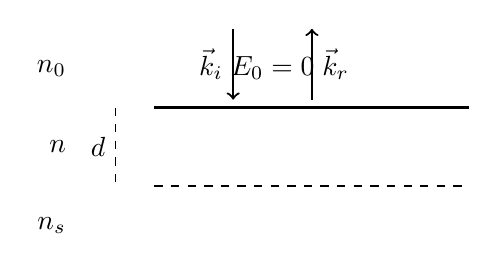
\begin{tikzpicture}[scale=1]
		% Regions
		\node[left] at (-1, 1) {$n_0$};
		\node[left] at (-1, 0) {$n$};
		\node[left] at (-1, -1) {$n_s$};
		
		\draw[thick] (0, 0.5) -- (4, 0.5);
		\draw[thick, dashed] (0, -0.5) -- (4, -0.5);
		\draw[dashed] (-0.5, 0.5) -- (-0.5, -0.5) node[midway, left] {$d$};
		
		% Vectors
		\draw[thick, ->] (1, 1.5) -- (1, 0.6) node[midway, left] {$\vec{k}_i$};
		\draw[thick, ->] (2, 0.6) -- (2, 1.5) node[midway, right] {$\vec{k}_r$};
		\node at (1.5, 1) {$E_0 = 0$};
	\end{tikzpicture}
\end{figure}

В среде $n_0$: $E_0 = E_i + E_r = 0$, $B_0 = \frac{n_0}{c}(E_i - E_r)$.
После прохождения тонкой пленки:
\begin{align*}
	\binom{E_t}{B_t} &= \begin{pmatrix} A & B \\ C & D \end{pmatrix} \binom{E_0}{B_0} \\
	\binom{E_t}{\frac{n_s}{c}E_t} &= \begin{pmatrix} A & B \\ C & D \end{pmatrix} \binom{E_i + E_r}{\frac{n_0}{c}(E_i - E_r)}
\end{align*}

Запишем систему:
\begin{equation}
	\begin{cases}
		E_t = A(E_i + E_r) + B \frac{n_0}{c}(E_i - E_r) \\
		\frac{n_s}{c}E_t = C(E_i + E_r) + D \frac{n_0}{c}(E_i - E_r)
	\end{cases}
\end{equation}

Ответ для коэффициента отражения $r = \frac{E_r}{E_i}$:
\begin{align*}
	r &= \frac{E_r}{E_i} = - \frac{\frac{n_s}{c}(A + \frac{n_0}{c}B) - (C + \frac{n_0}{c}D)}{\frac{n_s}{c}(A - \frac{n_0}{c}B) - (C - \frac{n_0}{c}D)} \\
	r &= - \frac{\frac{n_s}{c}(\cos kd - i\frac{n_0}{n}\sin kd) - (-i\frac{n}{c}\sin kd + \frac{n_0}{c}\cos kd)}{\frac{n_s}{c}(\cos kd + i\frac{n_0}{n}\sin kd) - (-i\frac{n}{c}\sin kd - \frac{n_0}{c}\cos kd)} \quad \qty(\text{скорость света $c$ сокращается}) \\
	r &= \frac{(n_s - n_0)\cos kd + i\sin kd \qty(\frac{n_0 n_s}{n} - n)}{(n_s + n_0)\cos kd + i\sin kd \qty(\frac{n_0 n_s}{n} + n)}
\end{align*}

Чтобы $r = 0$, необходимо: $\cos kd = 0$ и $\frac{n_0 n_s}{n} - n = 0$.
$$ kd = \frac{\pi}{2} \Rightarrow \frac{2\pi}{\lambda}d = \frac{\pi}{2} \Rightarrow d = \frac{\lambda}{4} \quad \text{(при такой толщине будет разность фаз $\pi$)} $$
$$ n = \sqrt{n_0 n_s} \quad \text{воздух } n_0 = 1 \Rightarrow n = \sqrt{n_s}. $$

\begin{example}{}{}
	\textbf{1. Матрица слоя $\frac{\lambda}{4}$:}
	$$ \hat{P}_1 = \begin{pmatrix} 0 & -i\frac{c}{n_1} \\ -i\frac{n_1}{c} & 0 \end{pmatrix} $$
	
	\textbf{2. Матрица пары слоев:}
	$$ \hat{P}_{12} = \begin{pmatrix} 0 & -i\frac{c}{n_2} \\ -i\frac{n_2}{c} & 0 \end{pmatrix} \begin{pmatrix} 0 & -i\frac{c}{n_1} \\ -i\frac{n_1}{c} & 0 \end{pmatrix} = \begin{pmatrix} -\frac{n_2}{n_1} & 0 \\ 0 & -\frac{n_1}{n_2} \end{pmatrix} $$
	
	\textbf{3. Для $N$ пар:}
	$$ \hat{P} = \begin{pmatrix} -\frac{n_2}{n_1} & 0 \\ 0 & -\frac{n_1}{n_2} \end{pmatrix}^N = \begin{pmatrix} \qty(-\frac{n_2}{n_1})^N & 0 \\ 0 & \qty(-\frac{n_1}{n_2})^N \end{pmatrix} $$
	
	Тогда коэффициент отражения:
	$$ r = -\frac{\frac{n_s}{c}A - \frac{n_0}{c}D}{\frac{n_s}{c}A + \frac{n_0}{c}D} = - \frac{n_s \qty(-\frac{n_2}{n_1})^N - n_0 \qty(-\frac{n_1}{n_2})^N}{n_s \qty(-\frac{n_2}{n_1})^N + n_0 \qty(-\frac{n_1}{n_2})^N} = \frac{\frac{n_s}{n_0}\qty(-\frac{n_2}{n_1})^{2N} - 1}{\frac{n_s}{n_0}\qty(-\frac{n_2}{n_1})^{2N} + 1} \xrightarrow{N \to \infty} 1 $$
\end{example}